% Created 2021-03-29 lun. 23:51
% Intended LaTeX compiler: pdflatex
\documentclass[a4paper,12pt]{article}
\usepackage[position=top,labelformat=empty]{subfig}
\usepackage{caption}
\usepackage[hmargin=2cm,vmargin=3cm]{geometry}


\usepackage{amsmath}
\usepackage{caption,graphicx,subcaption}
\usepackage[boxed]{algorithm2e}
\usepackage{authblk}
\author[1]{Vaitea Opuu}
\author[1]{Nono S. C. Merleau}
\author[1]{Matteo Smerlak}
\affil[1]{Max Planck Institute for Mathematics in the Sciences, D-04103 Leipzig, Germany}
\date{\today}
\title{A Mirror encoding and FFT for an RNA fast folding path heuristic}
\begin{document}

\maketitle
We propose an heuristic to the folding dynamic making use of a mirror encoding
and the fast Fourrier transform (FFT) called RAFFT. Based on simple folding
rules, it can create many parallel folding paths. The performance in the folding
task when compared to the state of the art folding tools were reasonable on a
well curated dataset. However, when all parallel folding paths were analyzed, it
revealed near native predictions (PVV \(\approx\) and sensitivity ) for sequences of
length below 200 nucleotides. In average, those predictions where found to be of
similar quality than recent deep-learning-based methods. The dynamics were built
with the stem-based rate model which displays coarse-grained folding paths.
Moreover, stems are sequentially added to the predicted structures if it
improves their overall stability. Those simple rules create smooth coarse
grained folding paths which are intuitive to analyze and gets along the
traditional two states view of the protein folding landscape and the fast
folding path concept. Hence, those paths could well approximate fast folding
paths. Since the algorithm was designed toward speed, it can be readily applied
to large RNAs.

\section{Introduction}
\label{sec:orgc76b153}
Natural RNA molecules as proteins have biologically relevant functions in
protein translation (mRNA, tRNA\ldots{}), but also in protein-like functions such as
where RNA can perform enzymes functions. Generally, those function can be better
understood through the light of their tri-dimensional structure. However, with
the discovery of riboswitch RNA molecules, the dynamic behavour of RNA is
getting more interest. Several other RNA system were found to allow multiple
metstable structures for highly tunable functions (\textbf{ref from kinwalker}).

RNA molecules are bio-polymers composed of nucleotides. These nucleotides are
simple molecules composed of a phosphate based backbone, a ribose, and a
variable nucleobase. Four different canonical bases/nucleobases compose the RNA,
namely adenine (A), guanine (G), uracyle (U), and cytosine (C). As proteins,
these nucleotide sequences can formed complex tri-dimensional structures which
allows their complex biological functions. Four main structure types are usually
considered: the primary structure which is the nucleotide sequence. The
secondary structure usually described by canonical base pairs interactions such
as G-C, A-U, and G-U. Next, the tertiary interactions involves other weaker
interactions within the same sequence. Finally, the quarternary structure is
defined by the interaction of multiple structured RNA molecules. However, unlike
proteins, these structures are usually hierarchically formed. The secondary
structure is generally formed first, then the tertiary structure is formed
(\textbf{ref}). Moreover, unlike proteins, the secondary structure provides an accurate
enough description of the thermodynamics and kinetics of RNA molecules. Although
base pairing can be formed with various configurations and depend on the base
side interactions (\textbf{ref, westhof}). It is possible to consider more coarse
grained interactions where the interaction geometries are not explicitly
considered. Many subtleties can be used to defined the secondary structure, but
we used here a well accepted formal definition called pseudoknot-free. This
forces the RNA to be drawable onto a plan where base pairs cannot cross (\textbf{ref}).
This has computational and theoretical benefits as will be described later.

The structure space of an RNA molecule is described by the stability of
individual possible structures. The stability \(\delta G_s\) of a structure \(s\) is
measured by the free energy changes with the completely unfolded state (no base
pairs). To predict secondary structures, thermodynamic methods use empirical
data to estimate RNA molecules stability. By assuming additivity (so
independant) of the loop contributions to the overall stability, NNM energy
model where developed (\textbf{ref}). It associates free energy values, determined by
optical melting experiments, to individual loop types and compositions. The
functional form allows for generalizable energy parameters, and it allows the
use of efficient dynamic programming algorithm capable of determining the
minimum free energy (MFE) structure. The MFE is considered as a gold standard
for the free-energy-based predictions. Other estimates exists such as the MEA,
however, it was found to be not significantly better than the MFE. Also, the MFE
has an intuitive intrepretation and is a strong concept with regards to the
folding landscape. Several tools implement such algorithm, named Zucker
algorithm (\textbf{ref}), such as RNAfold, Mfold, seqfold. Although those methods where
found to be consistently good at predicting RNA secondary structures, the
additivity foundation is expected to be doomed for large sequences and structure
complexifies. The non-additivity of tertiary interactions and pseudoknots
pairings can partially explained this discrepancy. Therefore, pseudoknots loop
contributions are not defined in the main paramters sets like the Turner2004
model. In addition, the thermodynamic energy models are not perfect. Another
limit of such prediction is the static picture that it gives to the RNA folding
landscape.

Therefore, kinetic information on RNA molecules were found to give valuable
complementary information (\textbf{riboswitch, regulatory}). To follow the dynamic of
individual RNA molecules, three rate models are currently used. The base stack
model uses base stacks formation and breaking as elementary moves (\textbf{ref}). The
base pair rate model uses base pairs as elementary steps as implemented in
kinfold (\textbf{ref}). kinfold implemented a continuous time Monte Carlo simulation to
simulate the RNA folding. It gives the finest resolution in the secondary
structure folding landscape but a the cost of computation time. The stem-based
model uses creation or deletion of stems to construct the folding dynamics. It
is among the first strategy explored (\textbf{ref}) and provides a coarse grained
description of the kinetic. The folding rates are therefore determined by the
free energy changes implied by the stem addition/removal. Although none of these
models where definitively rejected nor accepted, this ones makes a notable
assumption. Indeed, since transition states (or saddle points) hidden in the
formation of a given stem are not considered. An alternative approach,
implemented in kinwalker (\textbf{ref}), used the observation that folding paths are
generally composed of locally optimal conformations. Therefore, locally optimal
structures are formed using the standard dynamic programming algorithm and
aggregated together along the folding dynamic.

Here we propose a fast alternative for approximating fast folding paths based on
simple folding rules. It uses a mirror encoding and rely on the fast Fourrier
transform to speed up the search of stems. This method was inspired by MAFFT, a
well known multiple-alignment tool. Another FFT-based algorithm was already
developed, FFTbor2D, but uses the FFT differently. To assess the reliability of
the paths predicted, we compare its performance on the folding task for a well
curated dataset. The algorithm is compared to two estimates: the MFE computed by
RNAfold and a ML-based prediction computed by MxFold2. Next, we applied the
algorithm to a test case, the Coronavirus frameshifting stimulation element,
where it performed better than the MFE.

\section{FFT based folding dynamic heuristic}
\label{sec:org5175ba6}
We now describe the heuristic folding algorithm starting from one sequence S and
its associated unfolded structure of lenght L. We first create a numerical
representation of S where each type of nucleotide in replaced by a unit vector
of 4 components:
\begin{equation}
\begin{split}
A \rightarrow \begin{pmatrix} 1 0 0 0 \end{pmatrix}
U \rightarrow \begin{pmatrix} 0 0 0 1 \end{pmatrix}
C \rightarrow \begin{pmatrix} 0 1 0 0 \end{pmatrix}
G \rightarrow \begin{pmatrix} 0 0 1 0 \end{pmatrix}
\end{split}
\end{equation}
which gives us a \(4 \times L\) matrix we call X where each row is a nucleotide
type channel. Here, the first row would be the A channel which we refer to as
\(X^A\). Then, we create a second copy for which we revert the order of the
sequence and use the following complementary encoding:
\begin{equation}
\begin{split}
\bar{A} \rightarrow \begin{pmatrix} 0 0 0 w_{\scalebox{0.5}{AU}} \end{pmatrix}
\bar{U} \rightarrow \begin{pmatrix} w_{\scalebox{0.5}{AU}} w_{\scalebox{0.5}{GU}} 0 0 \end{pmatrix}
\bar{C} \rightarrow \begin{pmatrix} 0 0 w_{\scalebox{0.5}{GC}} 0 \end{pmatrix}
\bar{G} \rightarrow \begin{pmatrix} 0 w_{\scalebox{0.5}{GC}} 0 w_{\scalebox{0.5}{GU}} \end{pmatrix}
\end{split}
\end{equation}
where \(w_{AU}\), \(w_{GC}\), \(w_{GU\) are tunable parameters for the next step. We
call this new copy \bar{X}, the mirror of X.

For each of the 4 components, we compute the correlation between X and \bar{X}
and simply sum up the four channels to obtain the correlation between the two
copies:
\begin{equation}
cor(k) = (c_{X^A,\bar{X}^A}(k) + c_{X^U,\bar{X}^U}(k) + c_{X^G,\bar{X}^G}(k) + c_{X^C,\bar{X}^C}(k)) / min(k, 2 \times L-k)
\end{equation}
where \(c_{X^A,\bar{X}^A(k)\) is the correlation in the \(A\) channel between the
two copies. The correlation \(cor(k)\) gives the average number of base pairs for
a positional lag \(k\). One channel correlation between the copies is given by:
\begin{equation}
c_{X^A,\bar{X}^A}(k) = \sum\limits_{1\leq i \leq L, 1 \leq i + k \leq M} X^A(i) \times \bar{X}^A(i+k)
\end{equation}
where \(X^A(i)\) and \(\bar{X}^A(i+k)\) are the A channel of site \(i\) and \(i+k\).
X\textsuperscript{A}(i) \texttimes{} \bar{X}\textsuperscript{A}(i+k) is non zero if sites \(i\) and \(i+k\) can form a base
pair, and will be the value of the chosen weight as described above. Although
this operation requires \(O(N^2)\) operation, it can take advantage of the FFT
which reduces drastically its complexity to \(O(Nlog(N))\).

The large correlation values between the two copies indicates the positional lag
between at which the base pair density is high. Therefore, we use a sliding
window strategy to search for the longest consecutive base pairs within the
positional lag. Since the copies are symmetrical, we only need to slide over one
half of the positional lag. Once the longest base pairs are identified, we
simply compute the free energy change when those base pair are formed. We
perform the same search for the \(n\) highest correlation lags, which gives us \(n\)
possible possibilities. Then, we added to the current structure the base pairs
that gives the best change of energy.

We are now left with two segments, the interior and exterior of the group of
consecutive base pairs formed. The two exterior fragments are concatenated
together. Then, we simply apply recursively the same procedure on the two
segments separately in a "Breath First" fashion to form new consecutive base
pairs, until no base pair formation can improve the energy. However, it is
straightforward to consider pseudoknots by simply concatenating all the
fragments left.

The algorithm described so far tends to be stuck in the first local minima found
along the folding trajectory. To alleviate this, we propose a stacking procedure
where the 50 best trajectories are stored in a stack and evolved in parallel.
Hence, it offers the flexibility of overcoming some energy barriers. \textbf{Figure}
shows the whole procedure.

\section{Folding RNAs}
\label{sec:orgfdd6a76}
To evaluate the relevance of the folding dynamic heuristic, we compared the
algorithm performance for the folding task. In addition, to assess the effect of
sequence lengthens on these predictions, we analyzed their performance
length-wise.

\textbf{Figure} shows the performance in PPV and sensitivity for the four methods. It
shows that the ML method is consistently better than thermodynamic methods.
Length-wise T-test between the MFE and ML predicitons showed that this
difference is significant (pvalue \(\approx\) 10\textsuperscript{-12}) with a substantial
improvement of about 10\%. Although RAFFT predictions were found to be comparable
to MFE predictions, they are significantly less accurate (pvalue \(\approx\)
0.0002), with a drastic lost of performance for sequences of length greater than
300 nucleotides.

Among the 50 configurations produced by RAFFT, we found in average at least one
prediction with in average 59\% of PPV and <SENS> of sensitivity (blue curve in
\textbf{figure}). The overall gain of performances is not significantly different from
the MFE predictions. However, for the sequences of length lesser than 200
nucleotides, this gain was found to be substantial and significant (\(\approx\) 16 \%
better than the MFE). The accuracy for those sequences is equivalent to ML
performances. For sequence lengths greater than 300 nucleotides, we observed the
same drastic lost of accuracy, although we took only the best prediction among
the 50 saved configurations for each sequence.

Two regions of lack of performances were observed for all methods. A group of 28
sequences of length shorter than 80 nucleotides were evaluated with free of
their known structures about 9.8 kcal/mol greater than the MFE structures. Some
of them involve large exterior loop such as displayed in \textbf{figure}. The second
region is around 200 nucleotides length. The known structure of these sequences
also displayed large unpaired regions such as the one shown in \textbf{figure}.

\begin{figure}[!ht]
  \centering
  \subfloat[]{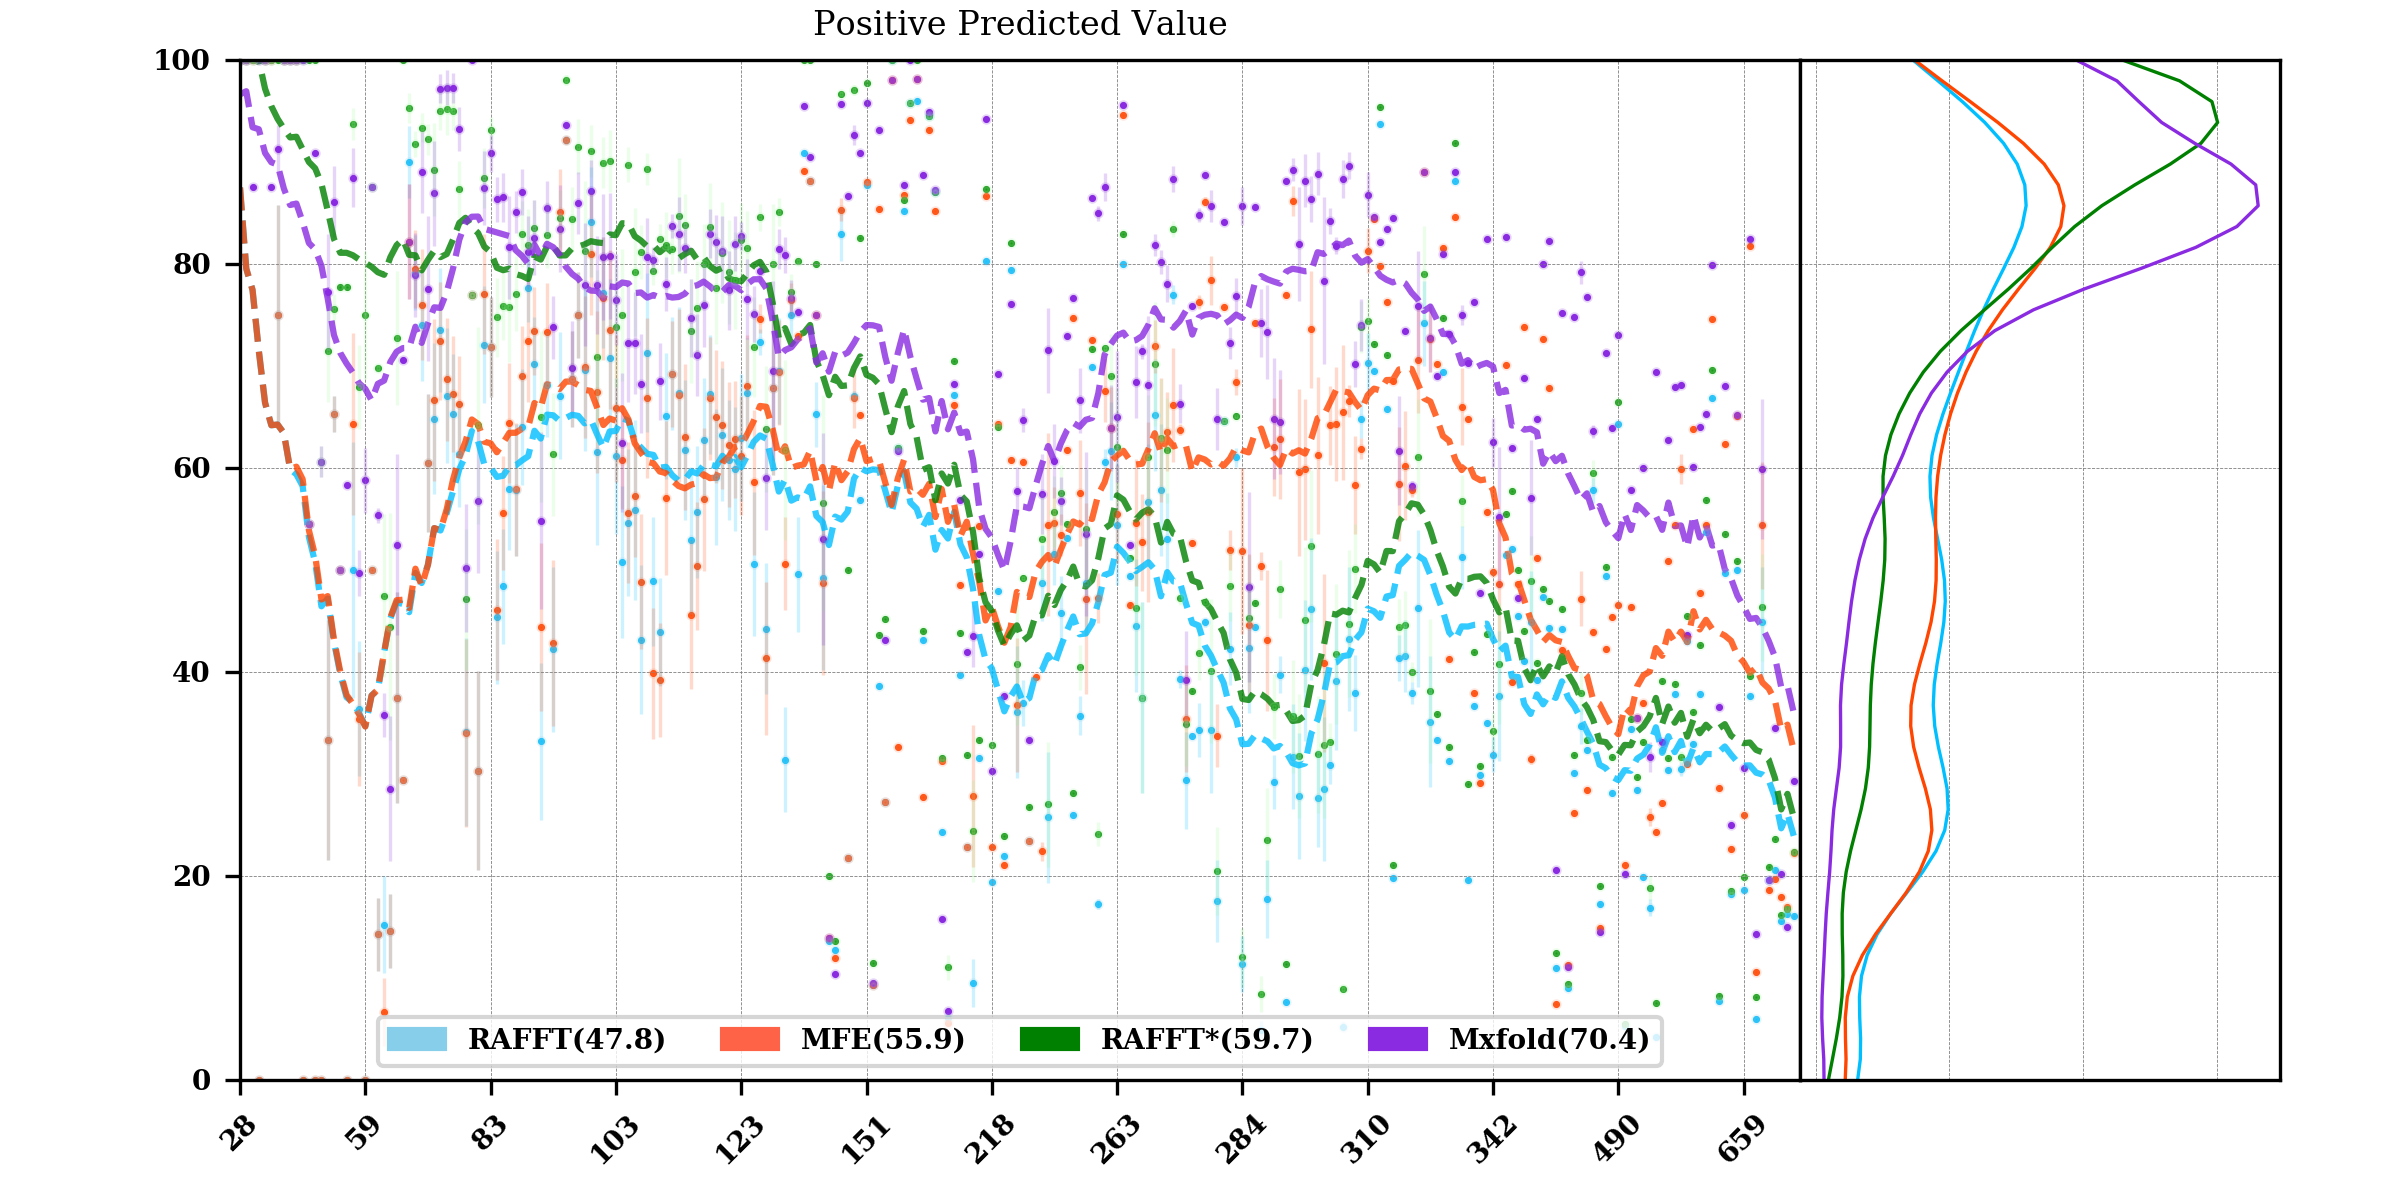
\includegraphics[scale=0.7]{img/fold_perf_pvv.png}}\\
  \subfloat[]{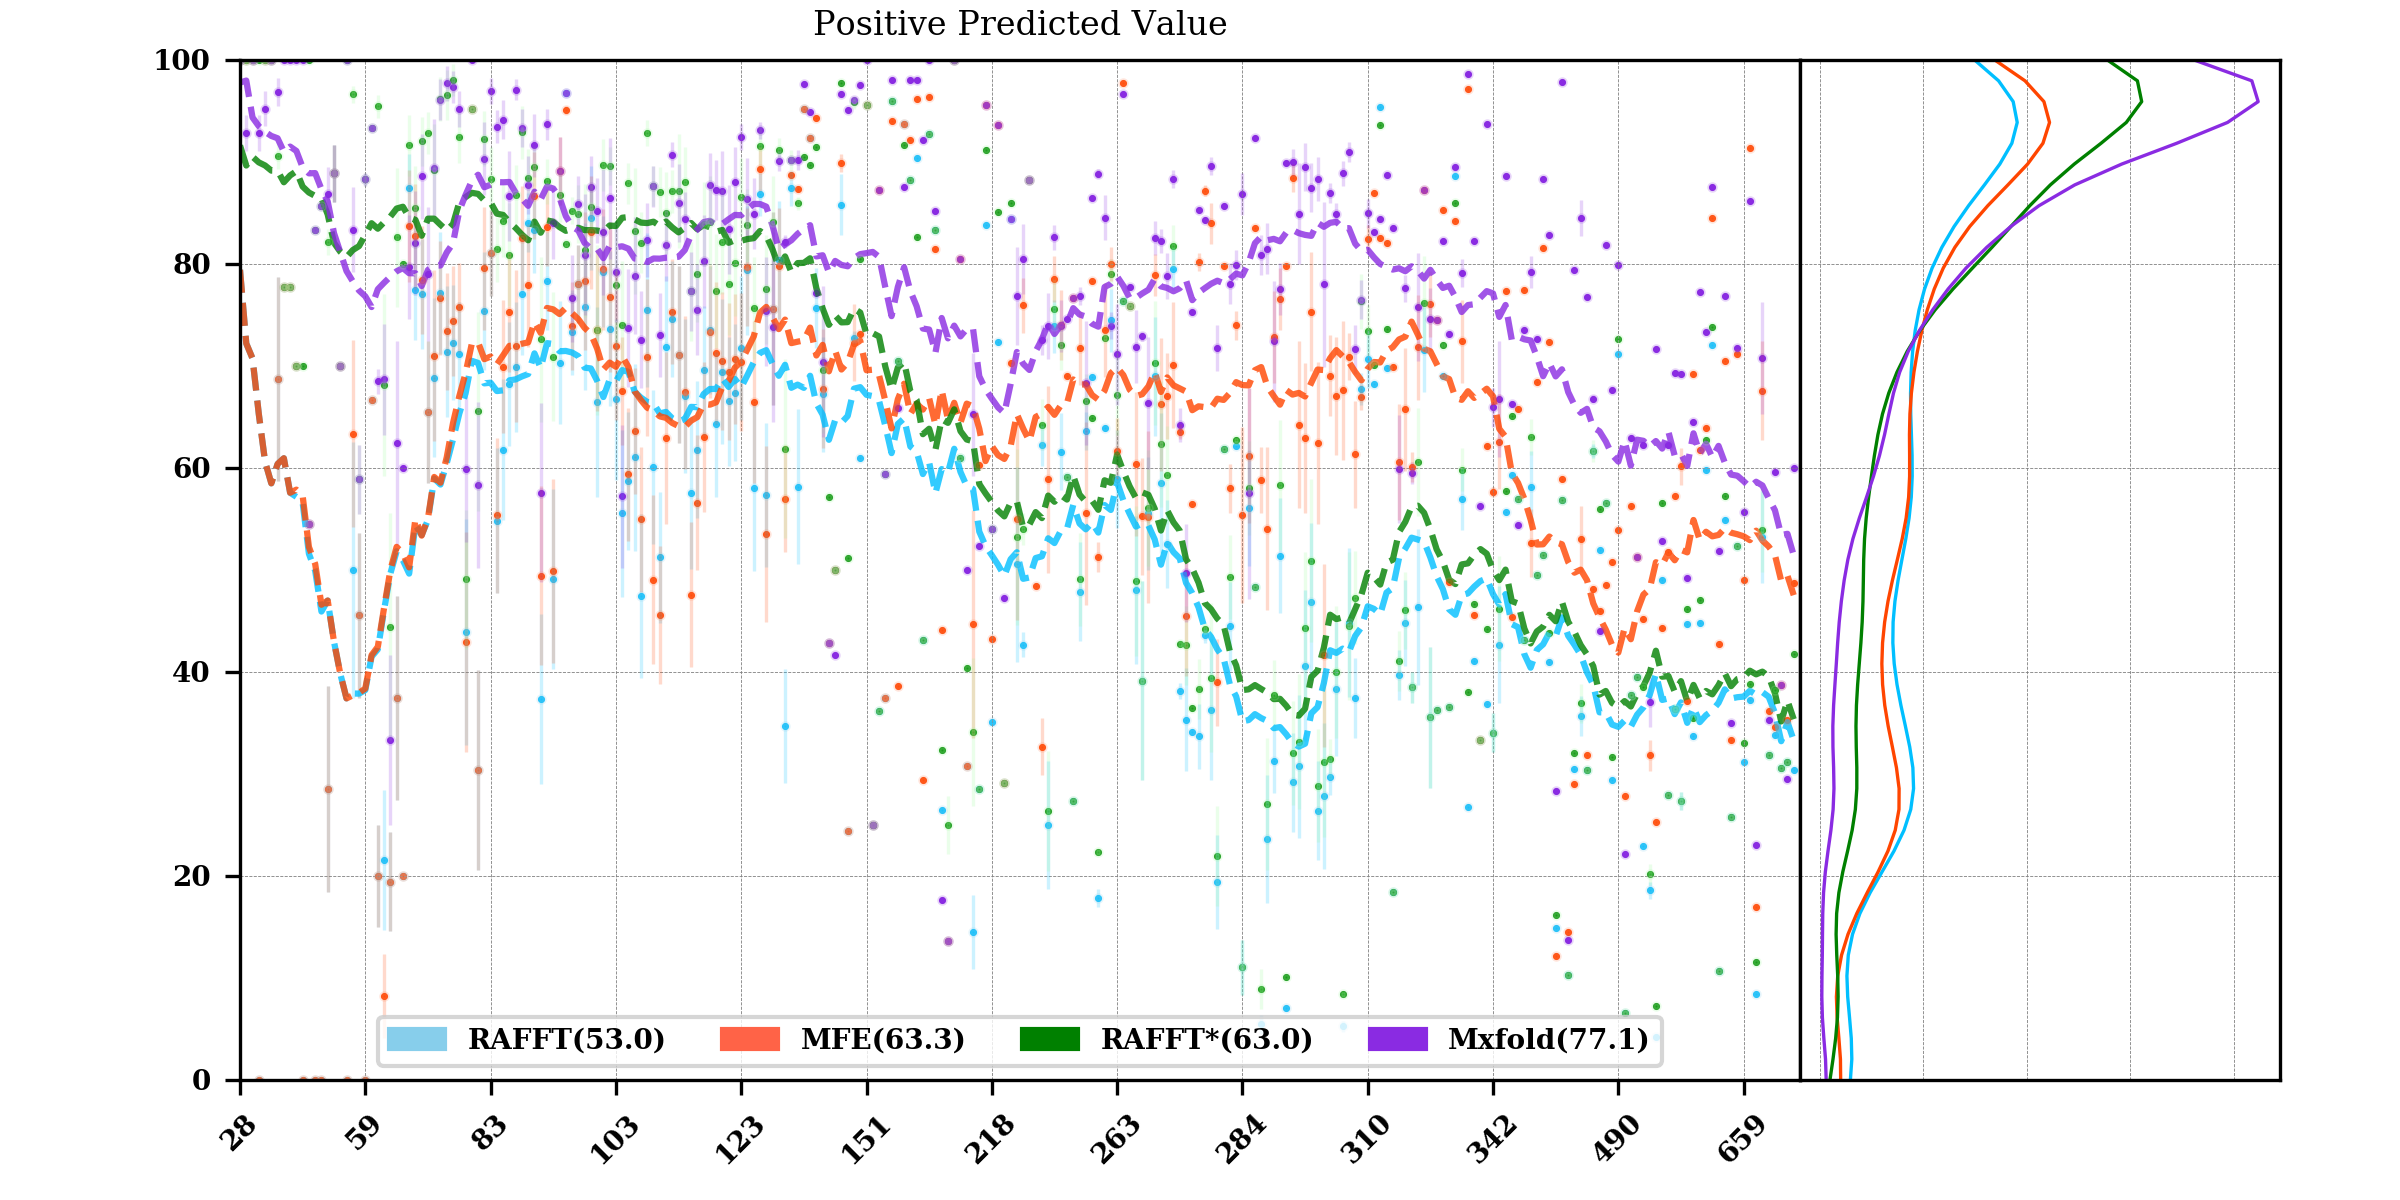
\includegraphics[scale=0.7]{img/fold_perf_sens.png}}
  \caption{\textbf{Predicted positive values and sensitivity results}}
\end{figure}

\begin{figure}[htbp]
\centering
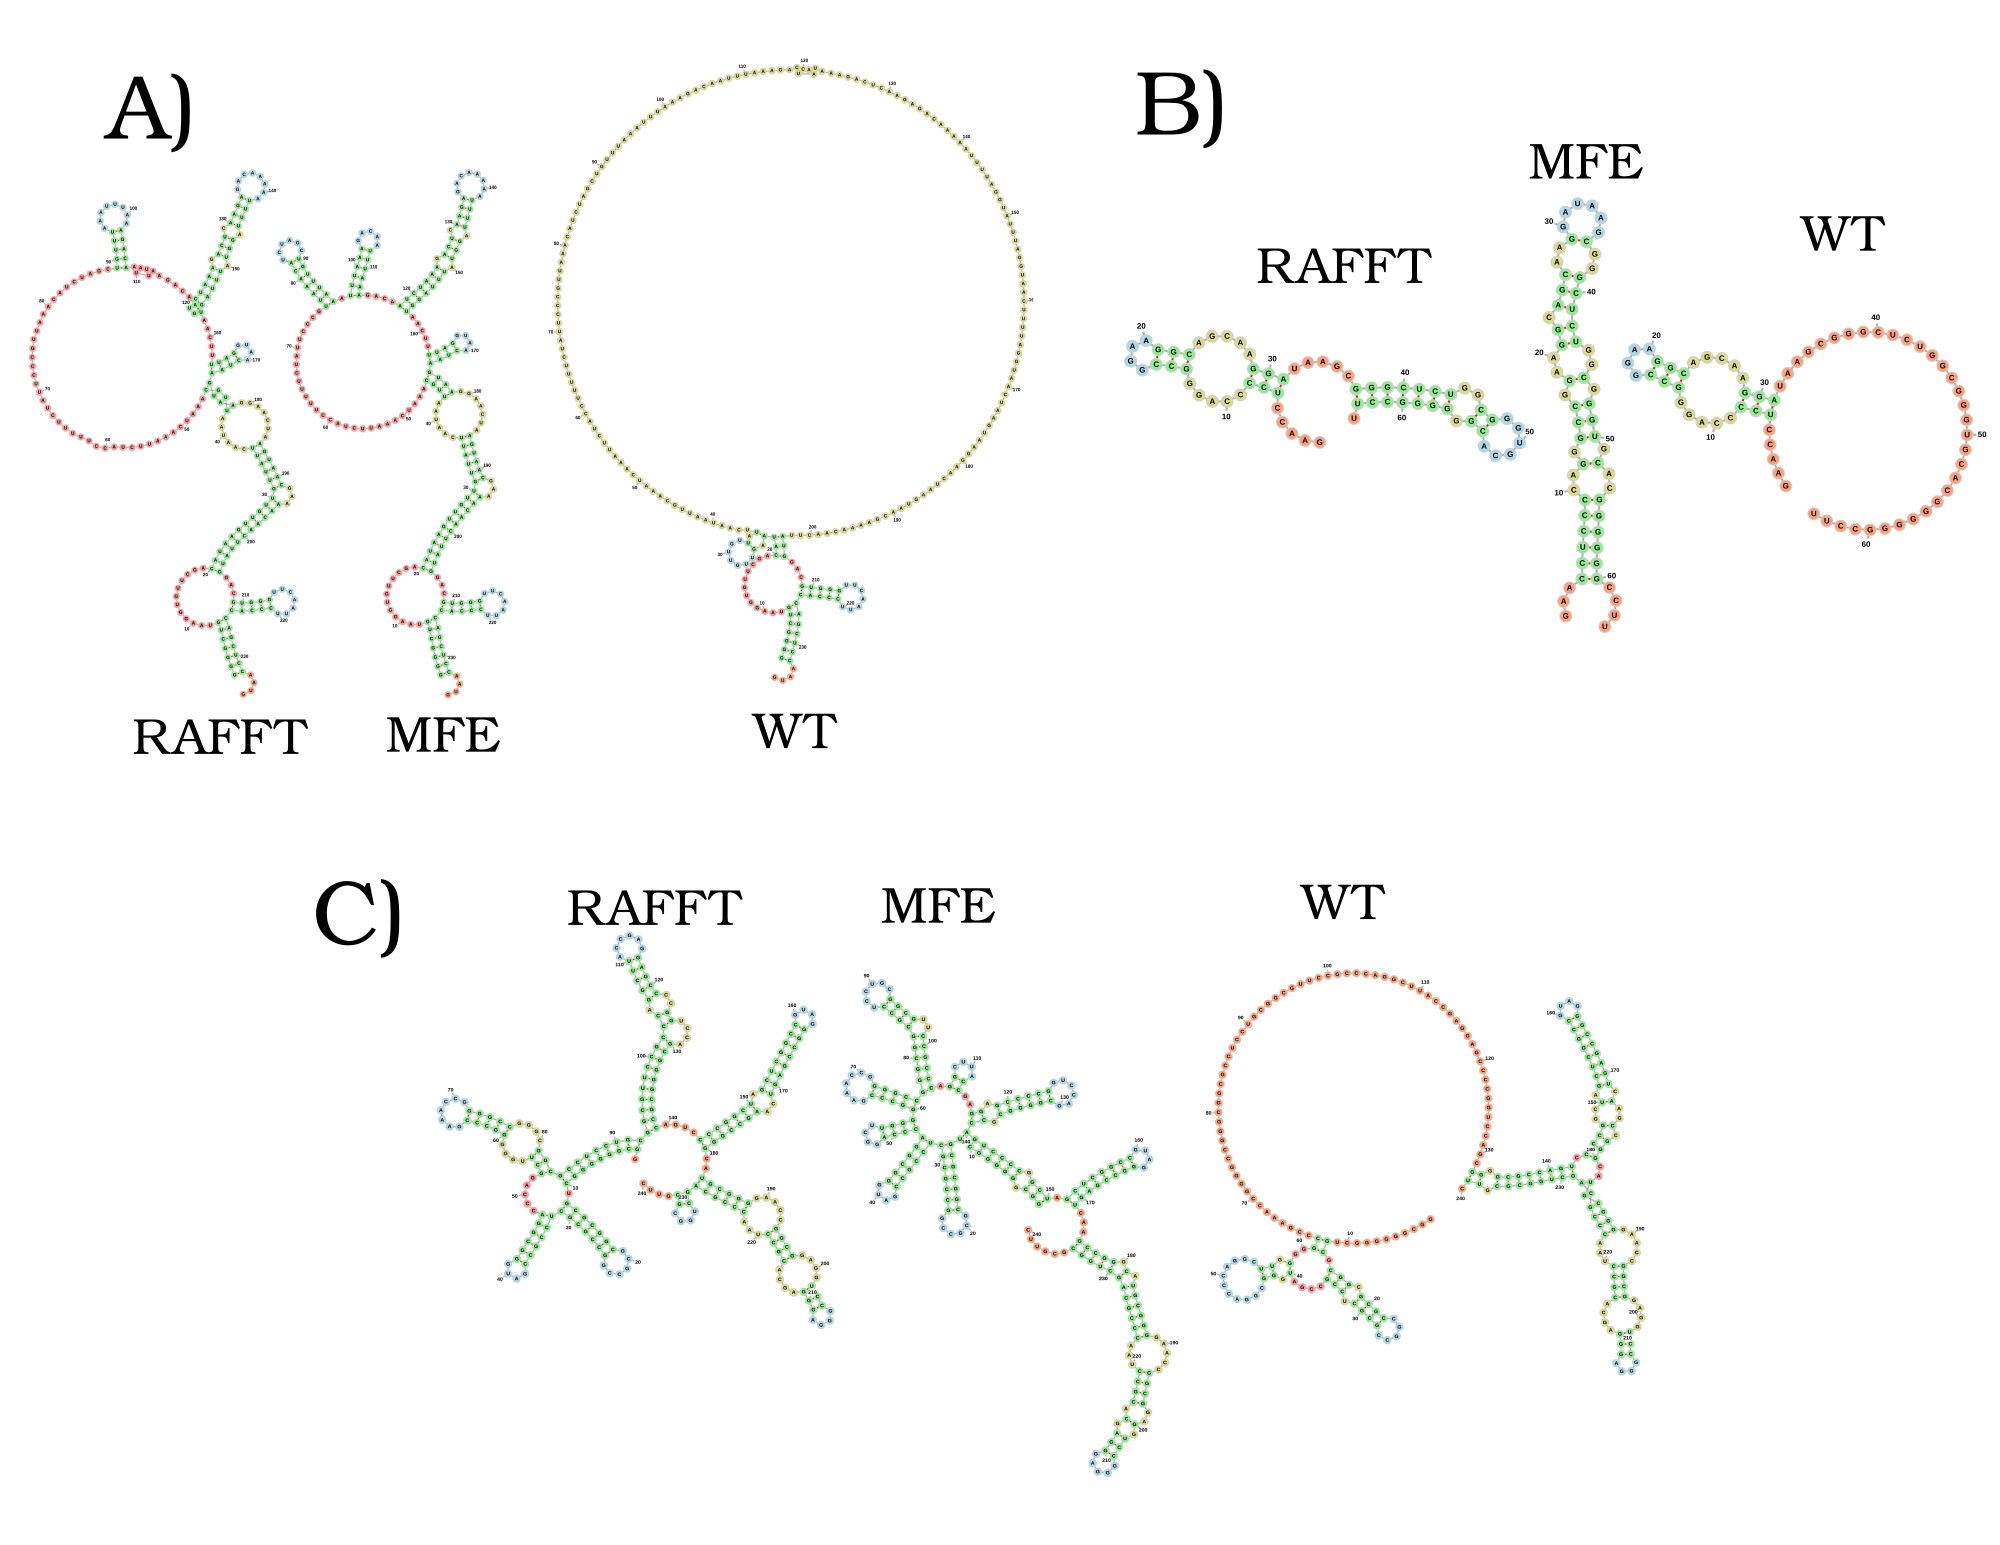
\includegraphics[width=.9\linewidth]{img/comb_rna_struct.png}
\caption{Difficult structures}
\end{figure}

To investigate the region of the structure space where the thermodynamic model
tends to fail, we computed the composition content of the known structures.
\textbf{Figure} shows the prcent of base pairs or positions involved in the five loop
types: interior, exterior, hairpin, stacking, and multi-branch loops. Those
prcents were then represented in a principal component analysis. From the PCA,
we observed that the known structures are distributed in the structure space
non-uniformly. Some natural structures, as observed above, have large exterior
loops. The center of mass in the principal component space is located in between
the high density stacking and interior loops. This shows that the dataset
contains many elongated structures.

\begin{figure}[htbp]
\centering
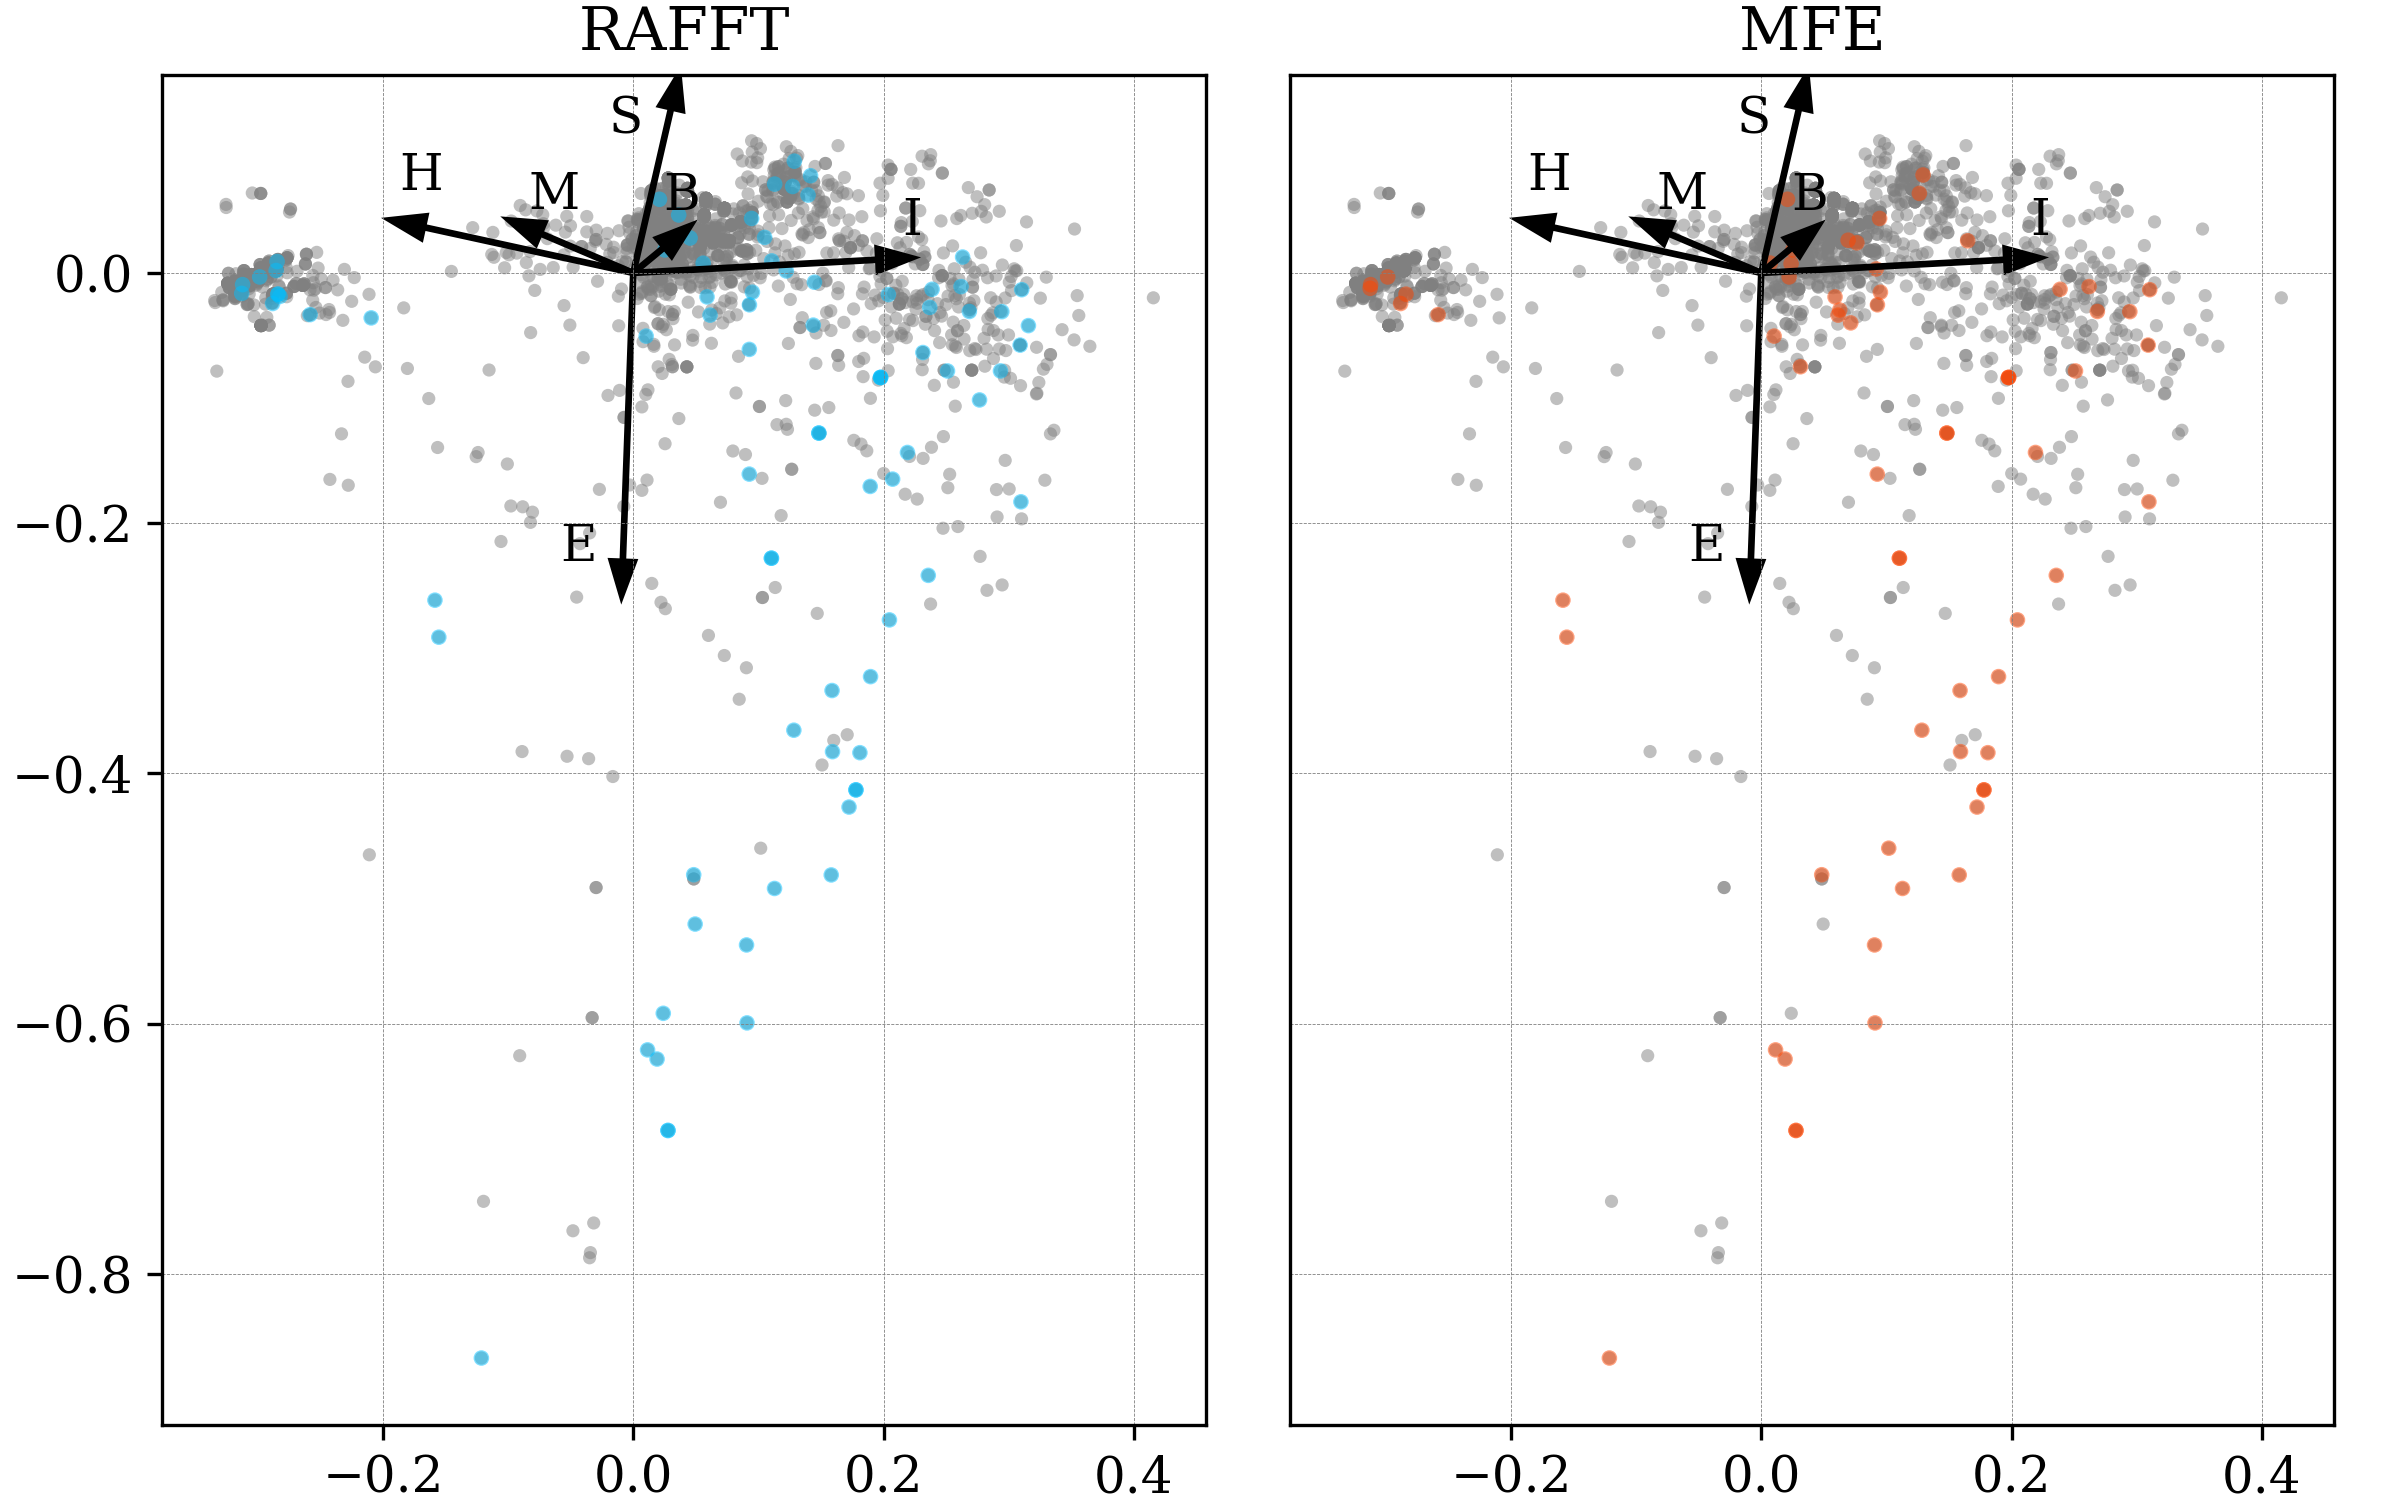
\includegraphics[width=.9\linewidth]{img/comp_fails.png}
\caption{where does the methods failed? PCA RNAfold, Mxfold, FFT, and}
\end{figure}

The thermodynamic model tends to produce more diverse structures as shown in
\textbf{figure}. Loops content were extracted from the predicted structures of each
method and projected onto their respective two first principal components space.
Both RAFFT and MFE predictions seems to produce a diverse structure space while
the ML method does allow for long unpaired regions in long hairpins.

\begin{figure}[htbp]
\centering
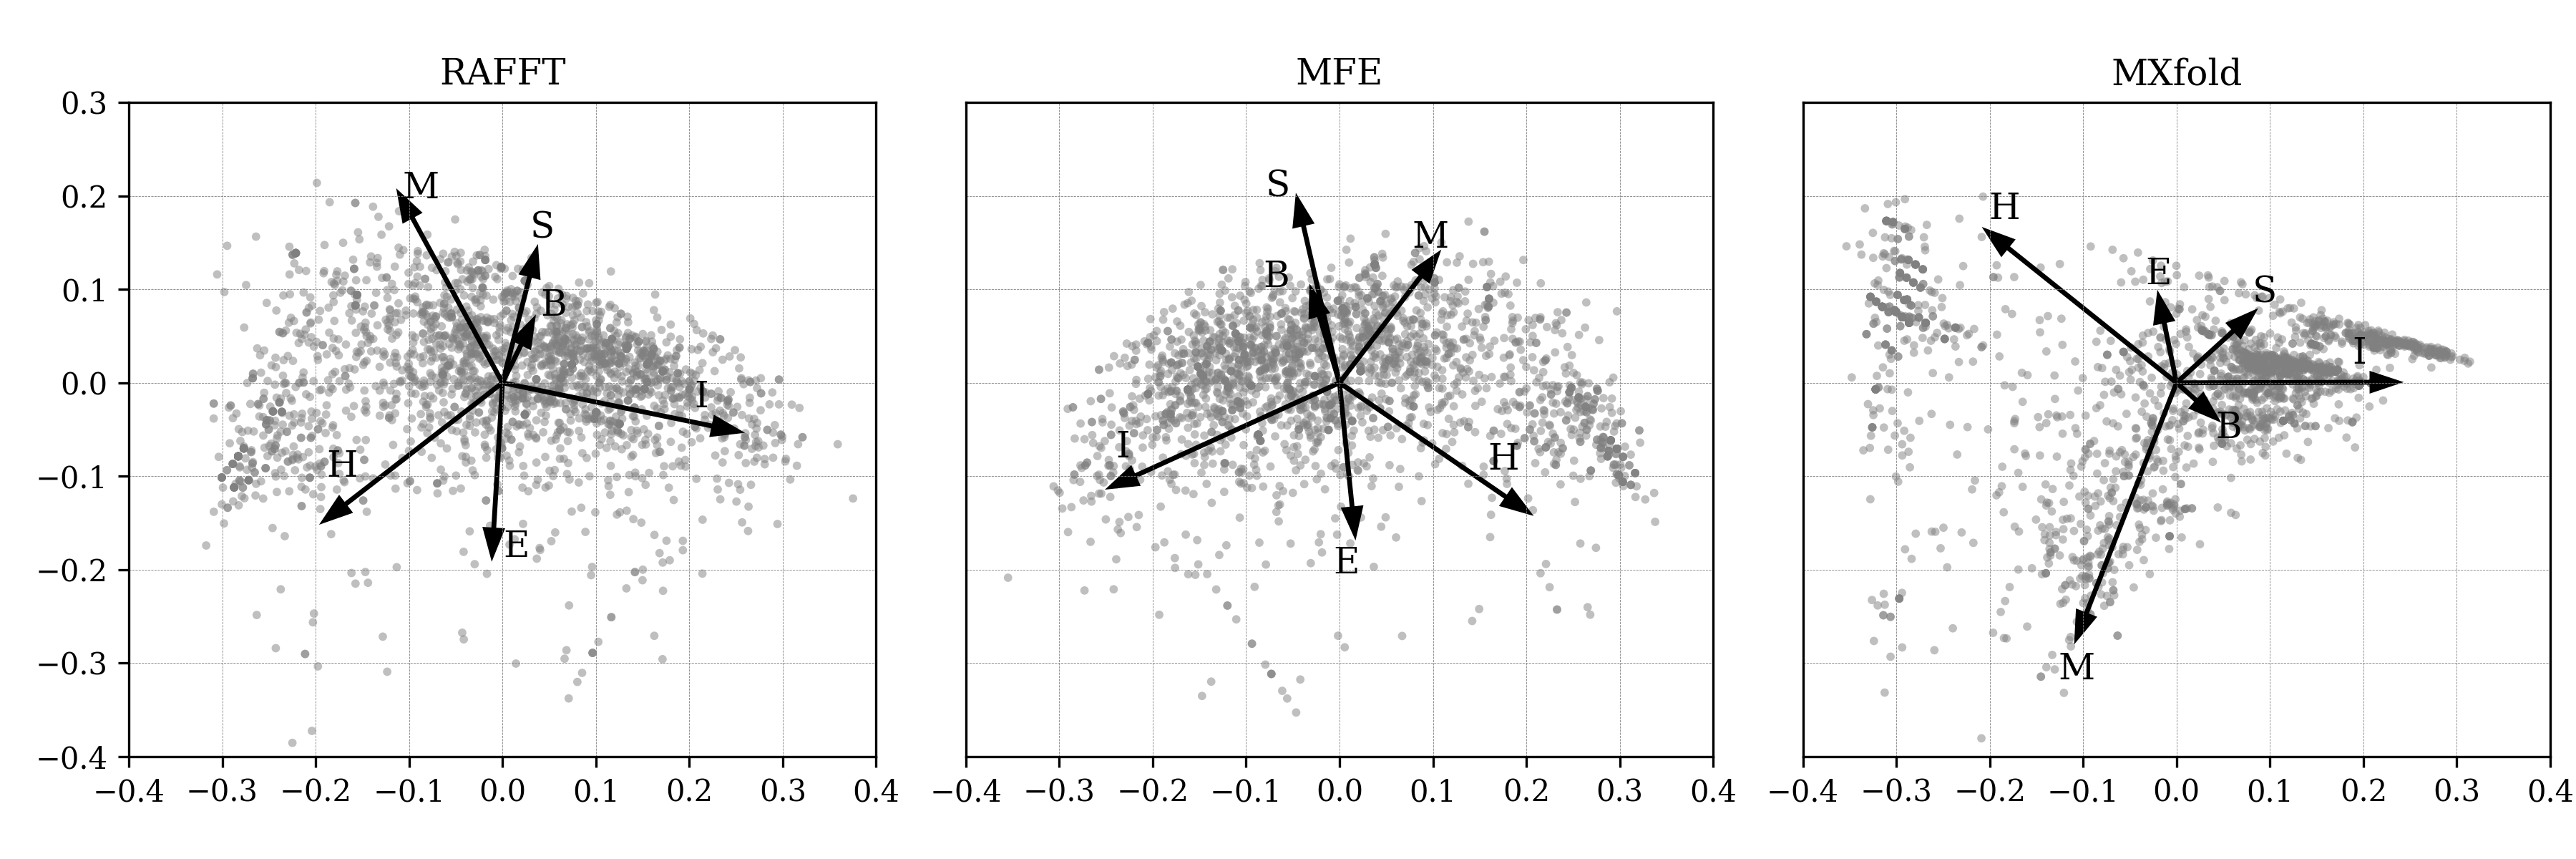
\includegraphics[width=.9\linewidth]{img/content_predicted_data.png}
\caption{What kind of structure these methods naturally produced}
\end{figure}

\begin{figure}[htbp]
\centering
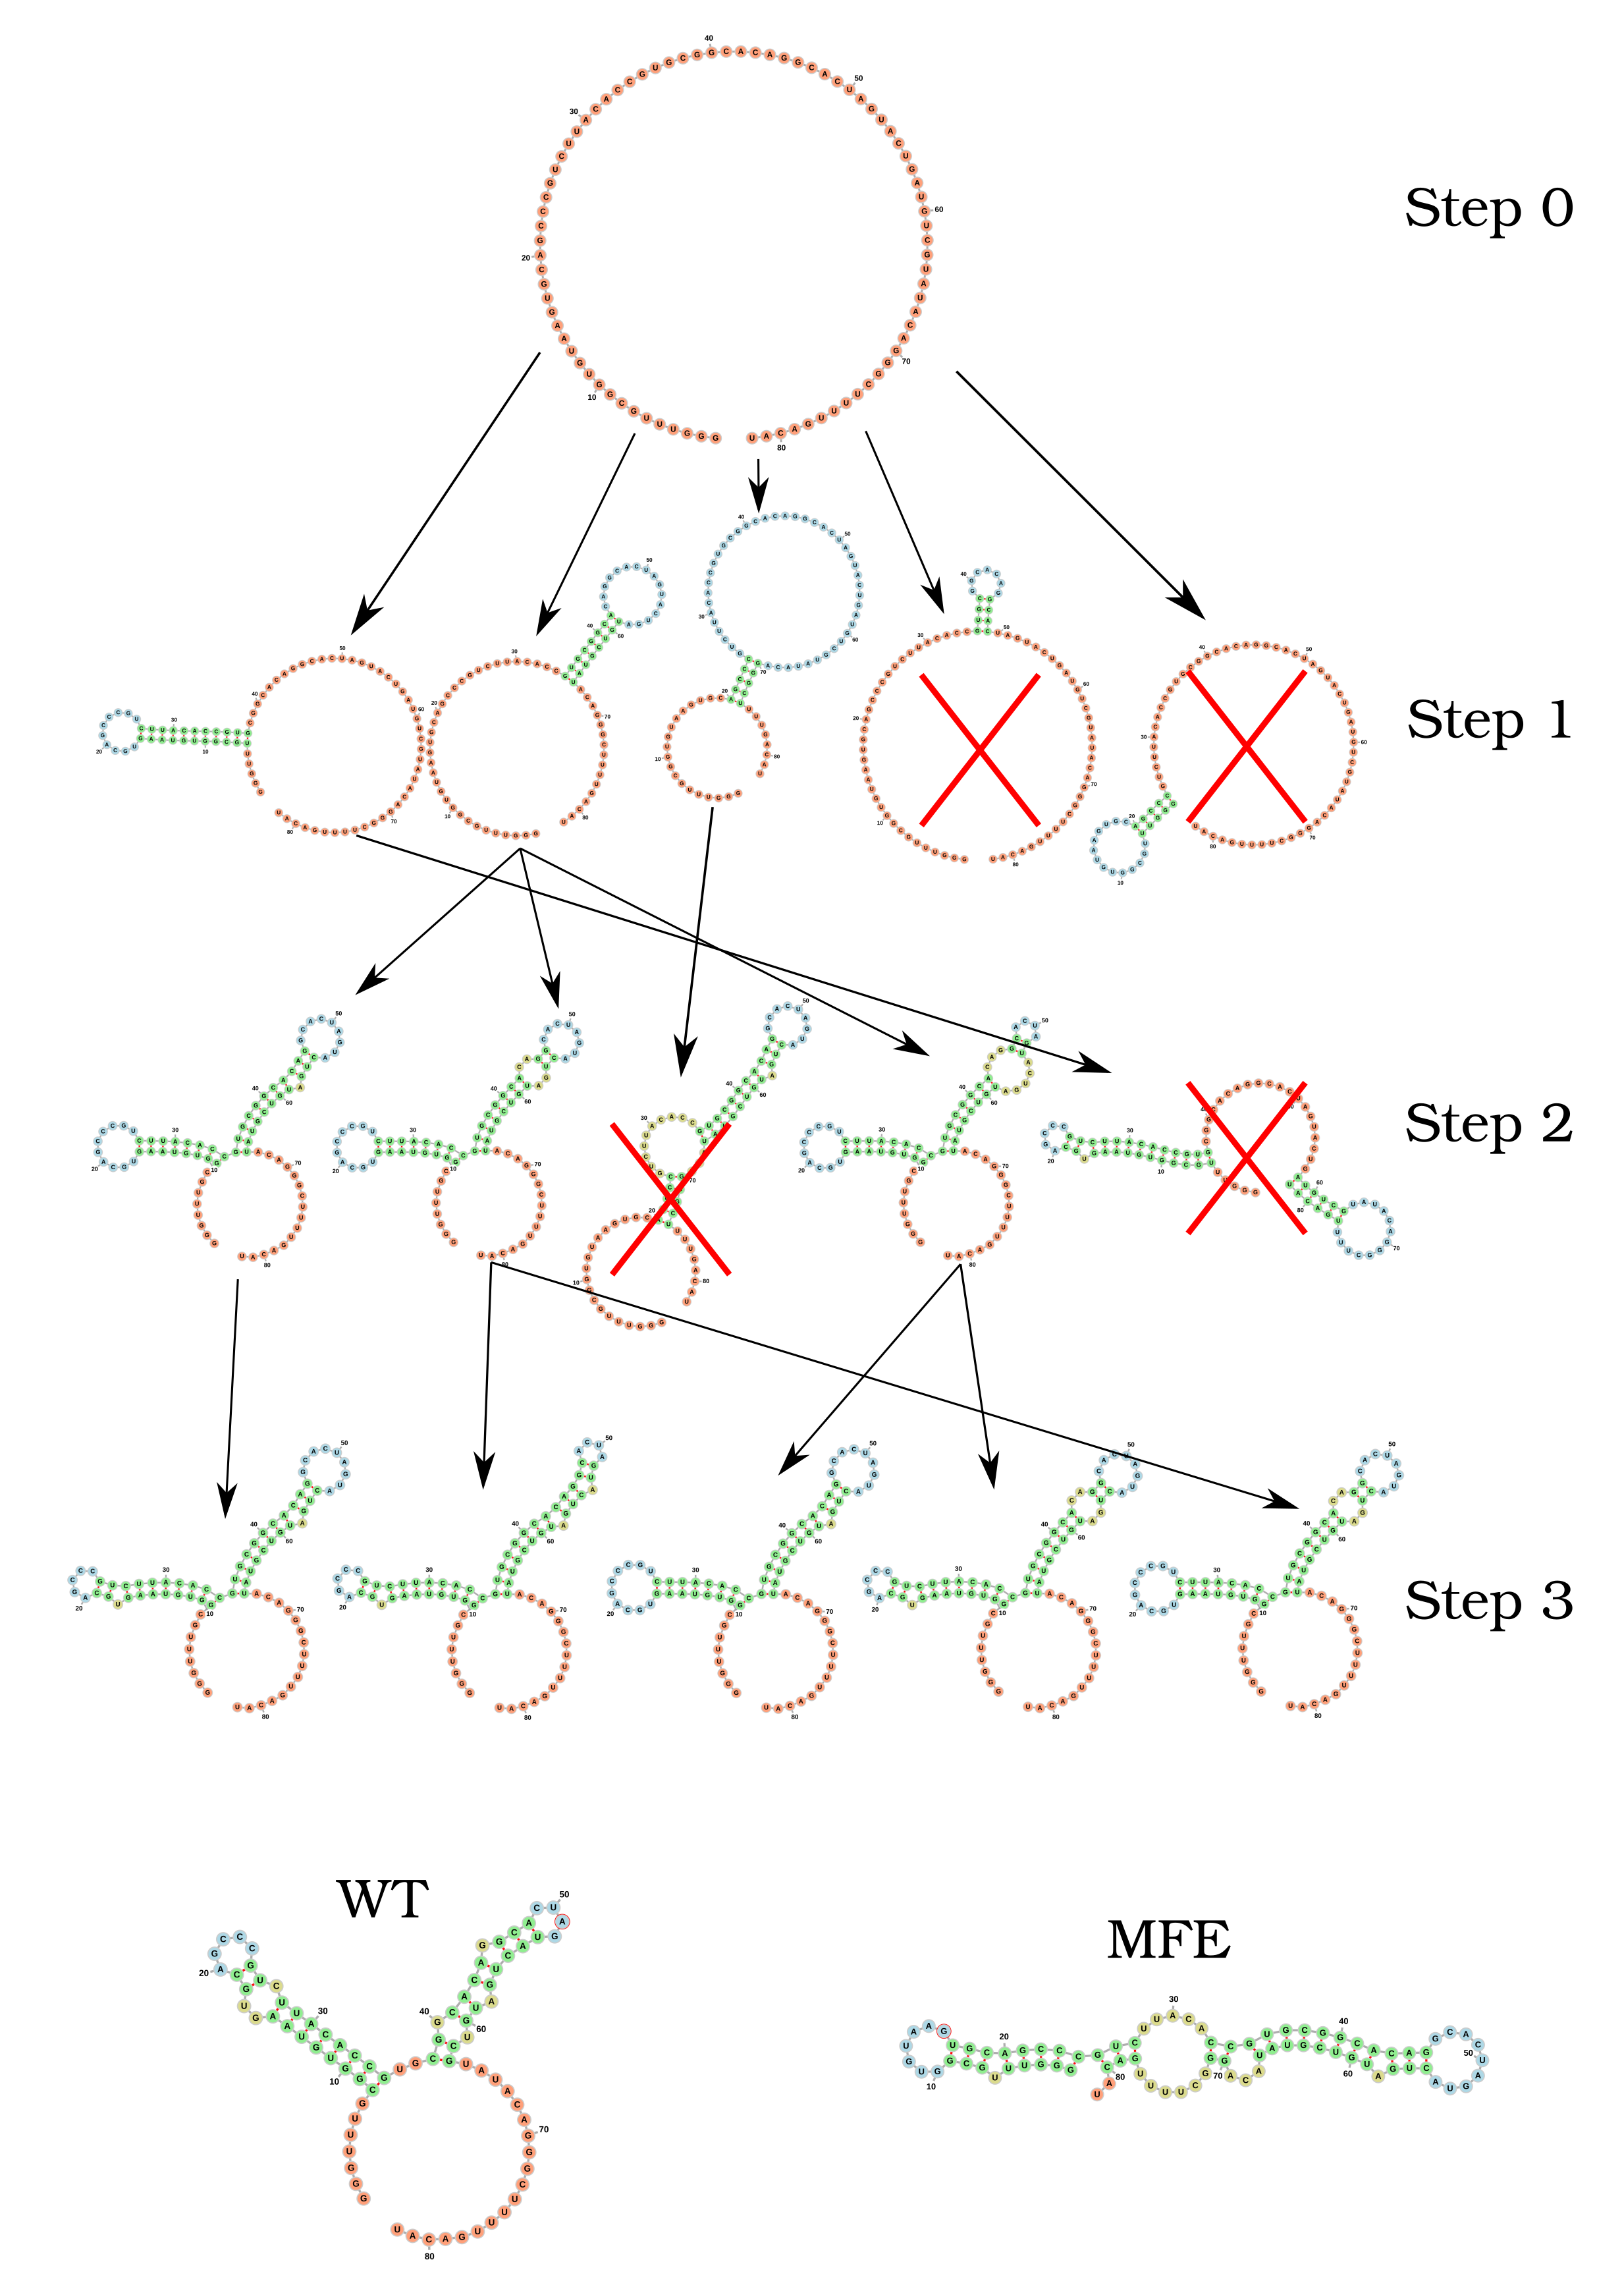
\includegraphics[width=.9\linewidth]{img/comb_frame_shift.png}
\caption{A folding trajectory example}
\end{figure}

\section{Concluding discussion}
\label{sec:orgccf874b}
We have proposed a simple heuristic of the RNA folding dynamic called RAFFT.
This heuristic uses a greedy rule to fold RNAs. Groups of consecutive base pairs
found to improve the energy are formed along the procedure in such a way a
smooth and coarse grained fashion. To search for consecutive base pairs, we
implemented a FFT-based technique which takes advantage of the mirror encoding.
Once a group of base pairs are formed, the sequence is split into two un-related
segments on which one can recursively search for new group of consecutive base
pairs. For one sequence, the algorithm can follow \(k\) folding paths. Finally,
the path which leads to the structure with the lowest energy is chosen.


To assess the relevance of the folding trajectories produced, we compared the
algorithm performance for the folding task. We considered three methods to
compare with: the MFE structure computed using RNAfold, the ML estimate using
MxFold tool and the kinetic approach using kinefold. Other thermodynamic-based
and ML-based tools where investigated but not shown here. We chose the MFE since
it provide a intuitive interpretation in the structure landscape, and the MEA
prediction was not found to be significantly more accurate (\textbf{ref how bench}).

From our experiments, RAFFT had an overall performance below the MFE predictions
by \(\approx\) 10\% of PVV and <SENS> of sensitivity. The ML-based approach dominated
the predictions (70.4\% of PPV and 77.7\% of sensitivity). We observed some
drastic lost of accuracies when the known structures contained large of unpaired
regions. These regions are unlikely to be stable and assumed to be very flexible
regions which could explain their presence. However, the effect of unpaired
regions seemed less dramatic for the ML method.

The principal component analysis performed on the known structure compositions
revealed a structure spaces prone to elongated structures were large unpaired
hairpins loops and exterior loops can be observed. The PCA analysis performed on
the structures predicted by the thermodynamic-based methods (RAFFT and MFE)
shown similar structure space, where flexible loops such as long hairpins or
exterior loops are of limited number. On the other hand, the ML method seemed to
be closer to the natural structure space. According to the thermodynamic model,
those unpaired regions have a local stability equal to zero. Hence, we suppose
that those regions are actually not stable in the sens that they don't have a
unique stable structure. However, the ML-method was able to identified such
structure more consistently than thermodynamic methods. This may suggest some
overfitting effects. We argue that not being able to recover such structures
would be a proof of robustness.

Although the overall performance of RAFFT was weak compared to the state of the
art in the folding task, we found one among the \(k=50\) predicted trajectories
that had a better accuracy than the low energy trajectory. In fact, the gain of
performance is substantial for the sequences of length lesser than 200
nucleotides with about 16\% better in PPV than the MFE predictions. The
performance is significantly similar to the ML-base method for that length
range. Sequences of length < 200 nucleotides represent 86.4\% of the total
dataset. However, for the 140 sequences of length greater than 300 nucleotides,
all \(k\) predictions per sequences were similar and performed worst than the
other methods.

Given the experiment results, we believe that RAFFT is a robust heuristic for
the folding dynamic since it can produce predictions of high accuracy for 86.4\%
of this dataset. The folding paths as calculated by RAFFT are smooth and coarse
grained since many base pairs, if it improves the energy, can be formed at once
and can lead to near-native structures. This near native coarse grained folding
path is an intuitive idea which get along with the funnel protein folding
landscape. We expect this heuristic to give valuable and complementary
information to the MFE-like predictions. However, some additional work are
necessary to determine whether the folding paths followed were experimentally
observed.

On the technical points, the mirror encoding as describe here is a versatile
tool for RNA analysis. Since it contains the relative positions of base pairs in
the whole sequence, we expect it to be extendable to other use cases such as
sequence clustering, or to the speed up of nussinov-like algorithms. On the
other hand, we are aware of the limits of chosing the maximal number of base
pairs each at each step. The greedyness of the algorithm as shown in \textbf{figure},
however, it had a limited impact on the results. We are not planning to provide
yet another folding tool, in this already crowded area of excellent softwares,
but one could combined this tool with a ML-base scoring for such a purpose.
\section{Methods}
\label{sec:orgea34db3}
We formed two sub-datasets based on the ArchiveII (\textbf{ref}) dataset. First, we
removed from all the structure containing pseudoknot since all tool considered
here don't handle pseudoknots. Next, we removed all the structures which were
evaluated with a positive energy or null energy with the Turner 2004 energy
parameters. Since positive energies means that the completely unfolded structure
is more stable than the native one, we assume that those structures are not well
modeled by the energy function used here. This dataset is composed of 2698
structures. 240 sequences were found multiple times (from 2 to 8 times). 19 of
them were found with different structures. We discarded all duplication and
picked the structure with the lowest energy for each. We obtained a dataset of
2296 sequences.

To compute the MFE structure, we used RNAfold (version) with the default
parameters and the Turner 2004 set of energy parameters. For the machine
learning tool, we computed the prediction using Mxfold2 with the default
parameters. The structures for both were used for the statistics.

For kinfold, we performed for each sequence, 40 simulations of 10\textsuperscript{4} (unit?).
Then, we counted the occurrences of each structures and selected the 50 most
populated structures. The best structure in terms of PPV was displayed and used
for the statistics.

For the FFT-based algorithm, we used two sets of parameters. First, we used
search for consecutive base pairs in the 50 best modes and stored 50
conformations for which we displayed the best energy found. The correlation were
computed using the weights w\textsubscript{GC}=3, w\textsubscript{AU}=2, and w\textsubscript{GU}=1.

To measure the predictions accuracy, we used two metrics from epimiology. The
positive predictive value (PPV) which is the fraction of correct base pairs
predictions in the predicted structure. The sensitivity is the fraction of
correctly predicted base pairs in the true structure. Both metrics are defined
as follow:
\begin{equation}
PPV = \frac{TP}{TP + FN} \;\;\; \text{Sensitivity} = \frac{TP}{TP+FP}
\end{equation}
where TP, FN, and FP stand respectively for the number of correctly predicted
base pairs (true positives), the number of base pairs not detected (false
negatives), and the number of wrongly predicted base pairs (false positives). To
maintain consistency with previous and future studies, we computed these metrics
using the implementation in the \texttt{scorer} tool provided in \textbf{ref Mathews}, which
provide also a more flexible estimate where shift are allowed.

The loop composition were extracted in terms of proportion to have an overall
measure of the structure distribution. We first convert all natural structures
into Shapiro notation using Vienna Package utilies. From the notation, we
extracted the proportion of base pairs involved into the interior, exterior,
bulge, stacking, and multibranch loops. For each true structure, we obtained a
prcent of type of loops from which we extracted the principal components. Next,
the structure compositions where projected on the first two principal components
for visual conveniences. The composition arrows represents the eigen vectors
obtained from the diagonalization of the covariance matrix.

\bibliographystyle{apalike}
\bibliography{../../bibliography/references}
\end{document}
